\documentclass[simplex.tex]{subfiles}
% DO NOT INCLUDE PREAMBLES/PACKAGES HERE!!
% packages are inherited from preamble.tex; you can compile this on its own
\begin{document}
\subsection{FlashX}

We re-implement Gaussian Mixture Model (GMM) in scikit-learn with FlashR,
which follows
the implementation in scikit-learn. This GMM implementation is much more
stable and mature than the previous one and supports covariance matrices
with different constraints. To demonstrate the speed and scalability of
our GMM implementation, we run our implementation on the k15f0 dataset,
which has over a million data points, and compare it against mclust.

\begin{table}
\begin{center}
\caption{Runtime of FlashR GMM vs. mclust on the k15f0 dataset with over
a million data points.}
\vspace{-10pt}
\footnotesize
\begin{tabular}{|c|c|c|c|c|}
\hline
& FlashR (min) & mclust \\
\hline
k=40, cov.type="full" & 11 & hours and fails to converge \\
\hline
k=10, cov.type="full" & 2.5 & hours and fails to converge \\
\hline
k=40, cov.type="diag" & 7.6 & hours and fails to converge \\
\hline
k=10, cov.type="diag" & 1.2 & hours and fails to converge \\
\hline
\end{tabular}
\normalsize
\label{tbl:GMM}
\end{center}
\vspace{-10pt}
\end{table}

\begin{figure}[!h]
\begin{cframed}
\centering
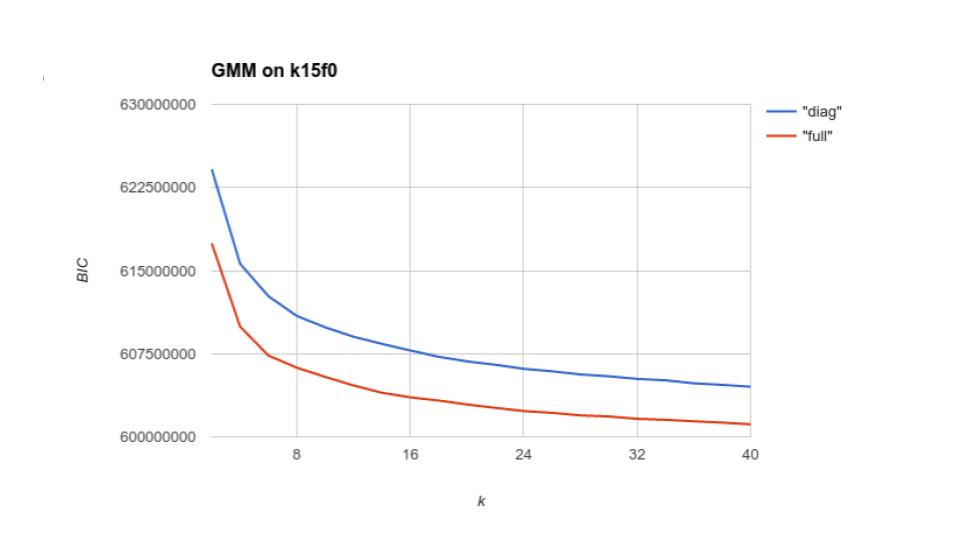
\includegraphics[width=0.6\textwidth]{../../figs/GMM.jpg}
\caption{Model selection for GMM on the dataset with BIC. We vary
the number of clusters (k) and the type of covariance matrices.
"diag" means diagonal covariance matrices and "full" means unconstrained
covariance matrices.}
\label{fig:FlashX2}
\end{cframed}
\end{figure}

\end{document}
